% Generated by code/scripts/report_figures.py at 2026-11-03T07:57:50Z; do not edit.
% Inputs: artifacts/local/runs/pipeline-e2e-20261103T075711Z/run
\begin{figure}[t]
\centering
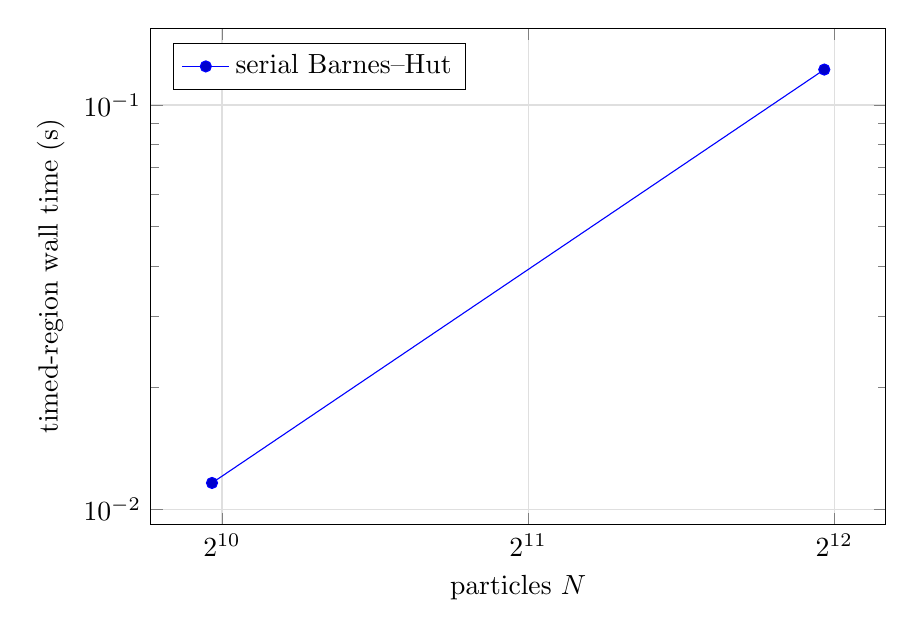
\begin{tikzpicture}
\begin{axis}[width=0.9\columnwidth, height=0.65\columnwidth, xlabel={particles $N$}, ylabel={timed-region wall time (s)}, xmode=log, log basis x=2, ymode=log, legend pos=north west, legend cell align=left, grid=major, grid style={gray!25}]
\addplot+[mark=*] coordinates {(1000,0.01161) (4000,0.1224)};
\addlegendentry{serial Barnes--Hut}
\end{axis}
\end{tikzpicture}
\caption{\textbf{LOCAL PIPELINE TEST, NOT A MEASUREMENT.} Serial runtime against problem size, $\theta=0.5$, leaf size 8, 2 timed steps, median of repetitions. Least-squares slope on the log--log axes: 1.699.}
\label{fig:serial-n}
\end{figure}
